\documentclass[12pt,a4paper]{article}
\usepackage[utf8]{inputenc}
\usepackage[english]{babel}
\usepackage{amsmath}
\usepackage{amsfonts}
\usepackage{amssymb}
\usepackage{makeidx}
\usepackage{graphicx}
\usepackage[left=2cm,right=2cm,top=2cm,bottom=2cm]{geometry}
\author{José Antonio García Hernández}
\title{14.4 Monte Carlo simulation of 2-d U(1) lattice gauge theory}
\begin{document}
\maketitle

We call $U_{\mu}(x)$ to a U(1) variable at point $x$ in the $\mu$ direction. For U(1), the lattice gauge action reads
\begin{equation}
	\label{eq:wilson_action}
	S[U] = \beta\sum_x \sum_{\mu < \nu} \text{Re}\  \left[1 - U_{\mu\nu}(x) \right],
\end{equation}
where $\beta = \frac{2}{e^2}$ and $e$ being the gauge coupling. The plaquettes are defined by
\begin{equation}
	\label{eq:plaquette}
	U_{\mu\nu}(x) = U_{\mu}(x)U_{\nu}(x+\hat{\mu})U_{\mu}^{\dagger}(x+\hat{\nu})U_{\nu}^{\dagger}(x) 
\end{equation}

The sum of plaquette variables is computed using 
\begin{equation}
	\label{eq:Sp}
	S_{\text{P}} =  \sum_x\sum_{\mu < \nu} \text{Re}\ U_{\mu\nu}(x),
\end{equation}
so the expectation value of an elementary Wilson loop or plaquette reads
\begin{equation}
	\label{eq:Ep}
	E_{\text{P}} =\frac{ \langle S_{\text{P}} \rangle}{D V},
\end{equation}
where $V=L^d$ is the volume of the lattice and $D = \frac{d(d-1)}{2}$ is the number of planes of rotation in $d$ dimensions.

We define the sum of staples as
\begin{equation}
	\label{eq:staples}
	\Sigma_{\mu}(x) = \sum_{\nu \neq \mu} \left[ U_{\nu}(x)U_{\mu}(x+\hat{\nu})U_{\nu}^{\dagger}(x+\hat{\mu}) + U_{\nu}^{\dagger}(x-\hat{\nu})U_{\mu}(x-\hat{\nu})U_{\nu}(x+\hat{\mu}-\hat{\nu})\right] .
\end{equation}


The change in the action  by a local update when changing $U_{\mu}(x) \to U'_{\mu}(x)$ is
\begin{equation}
	\label{eq:DS}
	\Delta S = -\beta \ \text{Re } \text{Tr} \left[ \left( U'_{\mu}(x) - U_{\mu}(x) \right)\Sigma_{\mu}^{\dagger}\right].
\end{equation}

We use the Metropolis algorithm for the simulation as decribed in the following steps:
\begin{enumerate}
	\item Given some gauge field configuration, we go through all the lattice points in a lexicographic way. At each point $x$ in the $\mu$ direction we generate a random U(1) variable $U'_{\mu}(x)$.
	
	\item We compute the sum of the staples and compute the change of the action according to eq.\ \eqref{eq:DS}. We generate a uniform random number $r\in [0,1)$ and accept the change if $r \leq p$, where $p$ is
	\begin{equation}
		p = \min (1, \exp(-\Delta S)).
\end{equation}	 
\end{enumerate}

	\begin{figure}
		\centering
		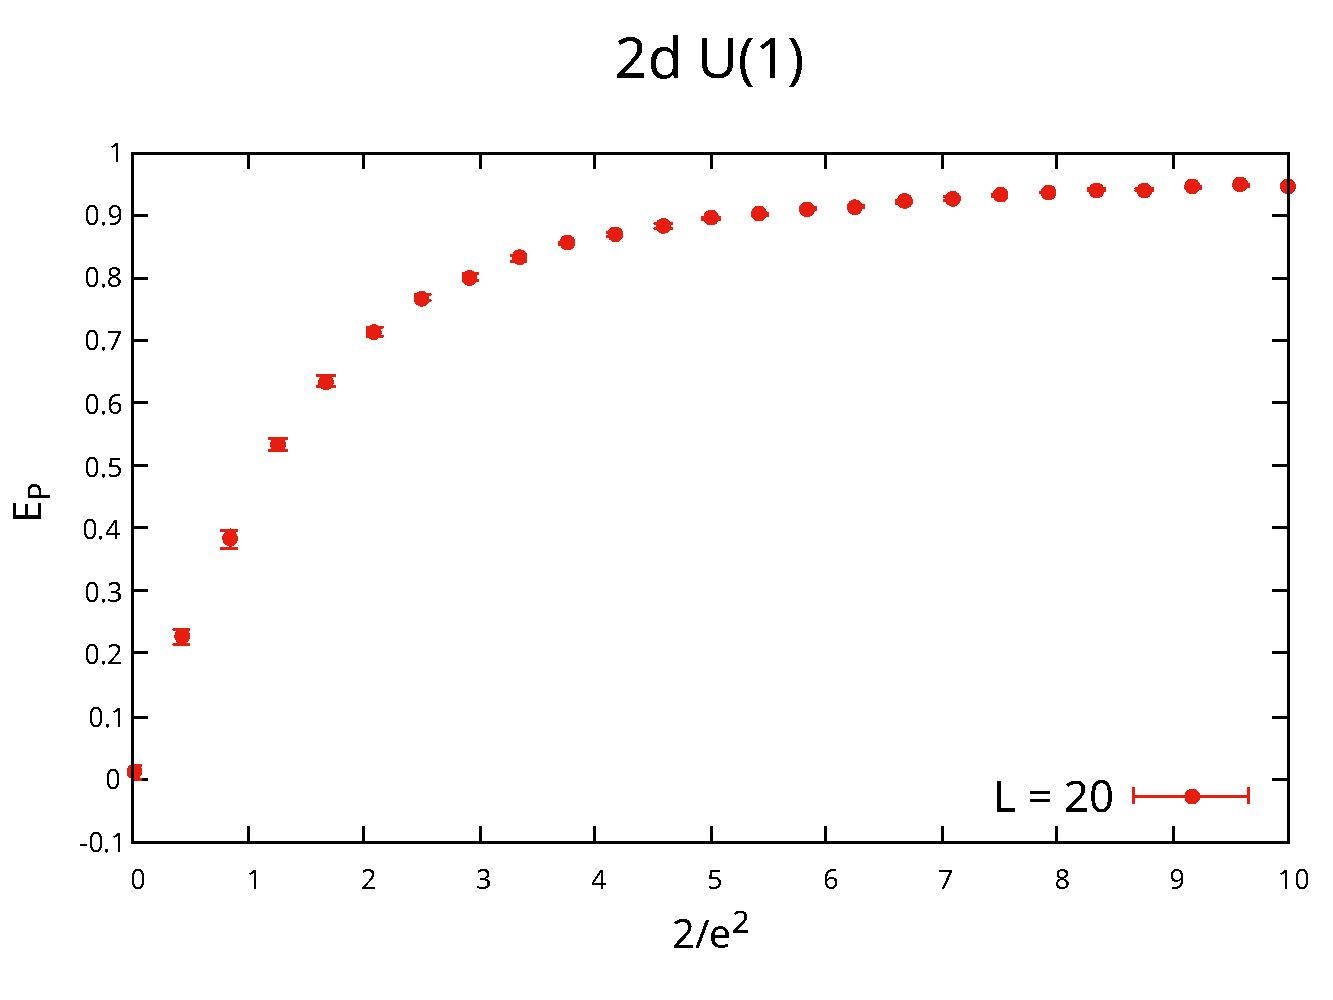
\includegraphics[scale=0.6]{n_term=1000-nmeas=5000-nskip=20.pdf}
		\caption{Expectation value of the plaquette variable vs.\ $\beta = 2/e^2$ with a volume $V = 20^2$. The errors were computed using the Jackknife error. The parameters of the simulation were: at each value of $\beta$, $5000$ measuremnts were made separated by 20 sweeps and a thermalization of 1000 sweeps.}
	\end{figure}

\end{document}
